\documentclass[portrait,final,a0paper,fontscale=0.28]{baposter}

\usepackage[vlined]{algorithm2e}
\usepackage{times}
\usepackage{calc}
\usepackage{url}
\usepackage{graphicx}
\usepackage{amsmath}
\usepackage{amssymb}
\usepackage{relsize}
\usepackage{multirow}
\usepackage{booktabs}
\usepackage[percent]{overpic}
\usepackage{graphicx}
\usepackage{multicol}
\usepackage{rotating}
\usepackage[T1]{fontenc}
\usepackage{ae}
\usepackage[lofdepth,lotdepth]{subfig}
\usepackage{wrapfig}
\usepackage{tabularx}

% see http://tex.stackexchange.com/questions/33039/using-ttfamily-with-bfseries-or-how-to-enable-bold-in-fixed-width-font
\usepackage[lighttt]{lmodern}

\newcolumntype{Y}{>{\centering\arraybackslash}X}

% see http://tex.stackexchange.com/questions/42619/x-mark-to-match-checkmark
\usepackage{amssymb}% http://ctan.org/pkg/amssymb
\usepackage{pifont}% http://ctan.org/pkg/pifont
\newcommand{\cmark}{\ding{51}}%
\newcommand{\xmark}{\ding{55}}%

% Remove "References" header from BibTex
% see http://tex.stackexchange.com/questions/132646/how-to-remove-the-references-title
\usepackage{etoolbox}
\patchcmd{\thebibliography}{\section*{\refname}}{}{}{}

\usepackage{tikz}
\usetikzlibrary{calc}
\usetikzlibrary{matrix}
\usetikzlibrary{arrows}
\usetikzlibrary{calc}
\usetikzlibrary{decorations.pathreplacing} % braces for tikz
\usetikzlibrary{positioning,shapes.geometric}
\usetikzlibrary{backgrounds}
\usepackage{mathtools}
\usepackage{pgfplots}
\usepackage{pgfplotstable}
\usepackage{multirow}

% using equal sign in column labels
\newcommand{\pgfequalsign}{=}
\newcommand\refbsdnyu[1]{% positions two related legendimages in one cell
  \raisebox{1.5pt}{\ref{plot:#1bsd}}\llap{\raisebox{-1pt}{\ref{plot:#1nyu}}}%
}

% TODO: FH black?
\pgfplotscreateplotcyclelist{comparison bsd}{%
	magenta,mark=star,solid\\% NC
	yellow!80!black,mark=star,solid\\% FH
	red!80!white,mark=star,solid\\% QS
	green!70!black,mark=star,solid\\% TP
	blue,mark=star,solid\\% SLIC
	%black,mark=star,solid\\% SLIC3D
	violet,mark=star,solid\\% CIS
	cyan,mark=star,solid\\% ERS
	brown!70!black,mark=star,solid\\% PB
	cyan,mark=star,dashed\\% SEEDS
	yellow!80!black,mark=star,dashed\\% reSEEDS
	%red!80!white,mark=star,dashed\\% reSEEDS3Dn
	%blue,mark=star,dashed\\% DASP
	green!70!black,mark=star,dashed\\% TPS
	violet,mark=star,dashed\\% CRS
	%brown!70!black,mark=star,dashed\\% VCCS
}
\pgfplotscreateplotcyclelist{comparison nyu}{%
	magenta,mark=star,solid\\% NC
	yellow!80!black,mark=star,solid\\% FH
	red!80!white,mark=star,solid\\% QS
	green!70!black,mark=star,solid\\% TP
	blue,mark=star,solid\\% SLIC
	%black,mark=star,solid\\% SLIC3D
	violet,mark=star,solid\\% CIS
	cyan,mark=star,solid\\% ERS
	brown!70!black,mark=star,solid\\% PB
	cyan,mark=star,dashed\\% SEEDS
	yellow!80!black,mark=star,dashed\\% reSEEDS
	red!80!white,mark=star,dashed\\% reSEEDS3Dn
	blue,mark=star,dashed\\% DASP
	green!70!black,mark=star,dashed\\% TPS
	violet,mark=star,dashed\\% CRS
	brown!70!black,mark=star,dashed\\% VCCS
}
\pgfplotscreateplotcyclelist{runtime nyu}{%
	%magenta,mark=star,solid\\% NC
	yellow!80!black,mark=star,solid\\% FH
	%red!80!white,mark=star,solid\\% QS
	%green!70!black,mark=star,solid\\% TP
	blue,mark=star,dotted\\% SLIC 1it
	blue,mark=star,solid\\% SLIC
	%black,mark=star,solid\\% SLIC3D
	%violet,mark=star,solid\\% CIS
	%cyan,mark=star,solid\\% ERS
	%brown!70!black,mark=star,solid\\% PB
	cyan,mark=star,dotted\\% SEEDS 1it
	cyan,mark=star,dashed\\% SEEDS
	yellow!80!black,mark=star,dotted\\% reSEEDS 1it
	yellow!80!black,mark=star,dashed\\% reSEEDS
	red!80!white,mark=star,dashed\\% reSEEDS3Dn
	blue,mark=star,dashed\\% DASP
	%green!70!black,mark=star,dashed\\% TPS
	%violet,mark=star,dashed\\% CRS
	brown!70!black,mark=star,dashed\\% VCCS
}

% \newcommand{\plotfontsize}{\scriptsize}

% http://tex.stackexchange.com/questions/207212/how-do-i-change-the-font-size-of-the-labels-along-the-axes-in-pgfplots
\pgfplotsset{tick label style={font=\tiny},every axis label/.append style={font=\tiny},}

\pgfplotsset{every axis/.append style={tick label style={/pgf/number format/fixed},font=\plotfontsize,ylabel near ticks,xlabel near ticks,grid=major}}
\pgfplotstableset{%
    highlightrow/.style={%
        postproc cell content/.append code={%
           \count0=\pgfplotstablerow
            \advance\count0 by1
            \ifnum\count0=#1
            %\pgfkeysalso{@cell content/.add={$\bf}{$}}
            \pgfkeysalso{@cell content=\textit{##1}}%
            \fi
        },
    },
}
\pgfplotstableset{%
  cignore row/.style={
    row predicate/.append code={
      \ifnum#1=\pgfplotstablerow\relax
        \pgfplotstableuserowfalse
      \fi
    }
  },
}

\makeatletter
\DeclareRobustCommand\onedot{\futurelet\@let@token\@onedot}
\def\@onedot{\ifx\@let@token.\else.\null\fi\xspace}
\def\eg{\emph{e.g}\onedot} \def\Eg{\emph{E.g}\onedot}
\def\ie{\emph{i.e}\onedot} \def\Ie{\emph{I.e}\onedot}
\def\cf{\emph{c.f}\onedot} \def\Cf{\emph{C.f}\onedot}
\def\etc{\emph{etc}\onedot} \def\vs{\emph{vs}\onedot}
\def\wrt{w.r.t\onedot} \def\dof{d.o.f\onedot}
\def\etal{\emph{et al}\onedot}
\makeatother

\begin{document}
\begin{poster}{eyecatcher=false}
% Eyecatcher
{
    
}
% Title
{
    \fontfamily{phv}\selectfont\Large Superpixel Segmentation: An Evaluation
}
% Authors
{
    \fontfamily{phv}\selectfont\normalsize \vspace*{5pt} David Stutz\\david.stutz@rwth-aachen.de
}
% University logo
{
    
\includegraphics[scale=0.14]{rwth_vci_weiss_rgb.png}
}
    
    \headerbox{Introduction}{name=introduction,column=0,span=1}{
       %  The term superpixel is used to describe a group of pixels similar in color or other low-level properties (Ren \etal, 2003). The concept is motivated by two aspects: pixels do not represent natural entities but are a result of discretization; and the usually high number of pixels prevents many algorithms from being computationally feasible.
       Superpixel algorithms have become a standard tool in computer vision. However, varying experimental setups and metrics used for evaluation make direct comparison difficult. We address this shortcoming with a thorough comparison of thirteen state-of-the-art superpixel algorithms including algorithms utilizing depth information.
    }
    
    \headerbox{Superpixel Algorithms}{name=algorithms,column=0,span=1,below=introduction,boxpaddingx=0em}{
        
        %{\footnotesize Table 1: Evaluated superpixel algorithms; M refers to MatLab.}
        %\vskip 0.25em
        
        \def\arraystretch{1.25}
        \begin{tabularx}{\textwidth}{l X c c c c}
            % \rowcolor{RWTHblue!60}& \multicolumn{1}{c}{\cellcolor{RWTHblue!60}\rotatebox{90}{Reference}} & \rotatebox{90}{Year} & \rotatebox{90}{Implementation\phantom{n}} & \rotatebox{90}{\#Superpixels} & \rotatebox{90}{Compactness} & \rotatebox{90}{Depth}\\\hline\hline
            % ------------------------------------------------------------------
            \multicolumn{5}{l}{\cellcolor{RWTHblue!50}\textbf{Superpixel algorithms}}\\\hline\hline
            \textbf{NC} & Ren \etal & 2003 & C/MatLab & \ref{plot:evaluation-comparison-nc-ue-nyu} \\ % \cite{RenMalik:2003}
            \rowcolor{RWTHblue!30}\textbf{FH} & Felzenswalb \etal & 2004 & C++ & \ref{plot:evaluation-comparison-fh-ue-nyu} \\ % \cite{FelzenswalbHuttenlocher:2004}
            \textbf{QS} & Vedaldi \etal & 2008 & C/MatLab & \ref{plot:evaluation-comparison-qs-ue-nyu}\\ %  \cite{VedaldiSoatto:2008}
            \rowcolor{RWTHblue!30}\textbf{TP} & Levinshtein \etal & 2009 & C/MatLab & \ref{plot:evaluation-comparison-tp-ue-nyu} \\ % \cite{LevinshteinStereKutulakosFleetDickinsonSiddiqi:2009}
            \textbf{SLIC} & Achanta \etal & 2010 & C++ & \ref{plot:evaluation-comparison-orislic-ue-nyu} \\ % \cite{AchantaShajiSmithLucchiFuaSuesstrunk:2010}
            \rowcolor{RWTHblue!30}\textbf{CIS} & Veksler \etal & 2010 & C++ & \ref{plot:evaluation-comparison-cis-ue-nyu} \\ % \cite{VekslerBoykovMehrani:2010}
            \textbf{ERS} & Liu \etal & 2011 & C++ & \ref{plot:evaluation-comparison-ers-ue-nyu} \\ % \cite{LiuTuzelRamalingamChellappa:2011}
            \rowcolor{RWTHblue!30}\textbf{PB} & Zhang \etal & 2011 & C++ & \ref{plot:evaluation-comparison-pb-ue-nyu} \\ % \cite{ZhangHartleyMashfordBurn:2011}
            \textbf{CRS} & Mester \etal & 2011 & C++ & \ref{plot:evaluation-comparison-crs-ue-nyu} \\ % \cite{MesterConradGuevara:2011}
            \rowcolor{RWTHblue!30}\textbf{SEEDS} & Van den Bergh \etal & 2012 & C++ & \ref{plot:evaluation-comparison-oriseedsmp-ue-nyu} \\ % \cite{VanDenBerghBoixRoigCapitaniVanGool:2012}
            \textbf{reSEEDS} & \textbf{SEEDS} reimplementation & -- & C++ & \ref{plot:evaluation-comparison-reseedssm-ue-nyu} \\
            \rowcolor{RWTHblue!30}\textbf{TPS} & Tang \etal & 2012 & C/MatLab & \ref{plot:evaluation-comparison-tps-ue-nyu} \\\addlinespace % \cite{DaiTangHuazhaFuXiaochunCao:2012}
            % ------------------------------------------------------------------
            \multicolumn{5}{l}{\cellcolor{RWTHblue!50}\textbf{Superpixel algorithms using depth information}}\\\hline\hline
             \textbf{reSEEDS3D} & \textbf{reSEEDS} using depth & -- & C++ & \ref{plot:evaluation-comparison-seeds3d-ue-nyu} \\
            \rowcolor{RWTHblue!30}\textbf{DASP} & Weikersdorfer \etal & 2012 & C++ & \ref{plot:evaluation-comparison-dasp-ue-nyu} \\ % \cite{WeikersdorferGossowBeetz:2012}
            \textbf{VCCS} & Papon \etal & 2013 & C++ & \ref{plot:evaluation-comparison-vccs-ue-nyu} \\ % \cite{PaponAbramovSchoelerWoergoetter:2013}
        \end{tabularx}
    }
    
    \headerbox{Datasets \& Benchmark}{name=datasets,column=0,span=1,below=algorithms}{
        \textbf{BSDS500} (Arbel\'{a}ez \etal, 2011)\textbf{.} 100 training and 200 test images of size 481 $\times$ 321.
        % 5 ground truth segmentations per image.
        \vskip 4pt
        
        \textbf{NYUV2} (Silberman \etal, 2012)\textbf{.} 200 training and 400 test images of size 608 $\times$ 448 including pre-processed depth.
        % semantic ground truth segmentations with instance labels.
        \vskip 4pt
        
        \textbf{Benchmark.} $N$ set of pixels; $G = \{G_i \subseteq N\}$ ground truth segmentation; $S = \{S_j \subseteq N\}$ superpixel segmentation; $TP(G,S)$, $FN(G,S)$ true positive and false negative boundary pixels.
        \vskip 2px
        
        
        {Boundary Recall}:
        \vskip -1em
        \begin{align}
            Rec(G, S) = \frac{|TP(G, S)|}{|FN(G, S)| + |TP(G, S)|}.\notag
        \end{align}
        
        {Undersegmentation Error}:
        \vskip -1em
        \begin{align}
            UE(G, S) = \frac{1}{|N|} \sum_{G_i \in G} \sum_{S_j \cap G_i \neq \emptyset} \min\{|S_j \cap G_i|, |S_j - G_i|\}.\notag
        \end{align}
    }
    
    \headerbox{Qualitative Results}{name=qualitative,column=0,span=1,below=datasets}{
        \begin{tabularx}{\linewidth}{@{}Y@{}Y@{}Y@{}Y@{}Y@{}Y@{}Y@{}}
            \resizebox{0.99\linewidth}{!}{
                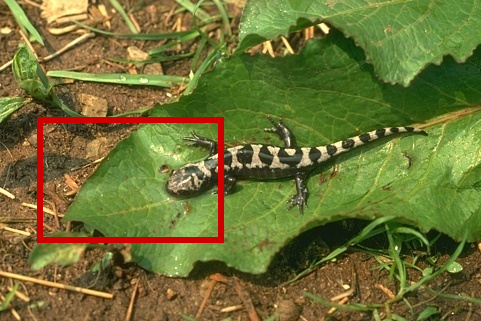
\includegraphics{../submission/pictures/bsd-test-2}
            }
            &
            %\resizebox{\linewidth}{!}{
            %    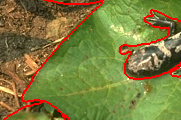
\includegraphics{../submission/pictures/bsd-test-2-contours-excerpt}
            %}
            %&
            \resizebox{\linewidth}{!}{
                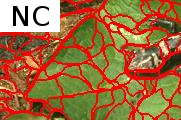
\includegraphics{../submission/pictures/bsd-test-2-nc-excerpt}
            }
            &
            \resizebox{\linewidth}{!}{
                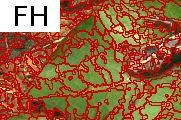
\includegraphics{../submission/pictures/bsd-test-2-fh-excerpt}
            }
            &
            \resizebox{\linewidth}{!}{
                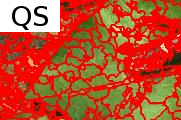
\includegraphics{../submission/pictures/bsd-test-2-qs-excerpt}
            }
            &
            \resizebox{\linewidth}{!}{
                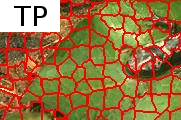
\includegraphics{../submission/pictures/bsd-test-2-tp-excerpt}
            }
            &
            \resizebox{\linewidth}{!}{
                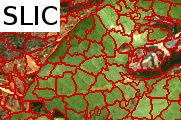
\includegraphics{../submission/pictures/bsd-test-2-orislic-excerpt}
            }
            &
            \resizebox{\linewidth}{!}{
                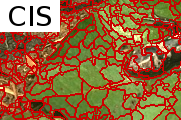
\includegraphics{../submission/pictures/bsd-test-2-cis-excerpt}
            }
            \\
            &
            \resizebox{\linewidth}{!}{
                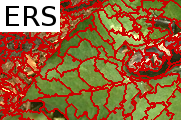
\includegraphics{../submission/pictures/bsd-test-2-ers-excerpt}
            }
            &
            \resizebox{\linewidth}{!}{
                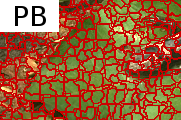
\includegraphics{../submission/pictures/bsd-test-2-pb-excerpt}
            }
            &
            \resizebox{\linewidth}{!}{
                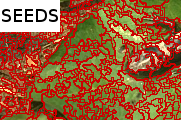
\includegraphics{../submission/pictures/bsd-test-2-oriseedsmp-excerpt}
            }
            &
            \resizebox{\linewidth}{!}{
                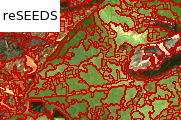
\includegraphics{../submission/pictures/bsd-test-2-reseedsmp-excerpt}
            }
            &
            \resizebox{\linewidth}{!}{
                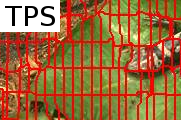
\includegraphics{../submission/pictures/bsd-test-2-tps-excerpt}
            }
            &
            \resizebox{\linewidth}{!}{
                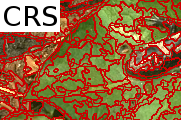
\includegraphics{../submission/pictures/bsd-test-2-crs-excerpt}
            }
        \end{tabularx}
        
        {\footnotesize Figure 1: Superpixel segmentations obtained on an image from the BSDS500.}
        \vskip 0.5em
        
        \begin{tabularx}{\linewidth}{@{}Y@{}Y@{}Y@{}Y@{}Y@{}Y@{}Y@{}Y@{}}
            \resizebox{0.99\linewidth}{!}{
                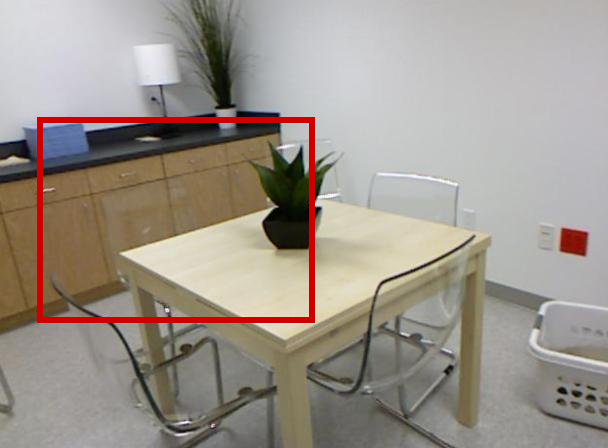
\includegraphics{../submission/pictures/nyu-test-1}
            }
            &
            %\resizebox{\linewidth}{!}{
            %    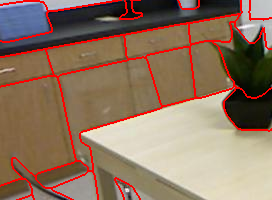
\includegraphics[scale=0.2016]{../submission/pictures/nyu-test-1-contours-excerpt}
            %}
            %&
            \resizebox{\linewidth}{!}{
                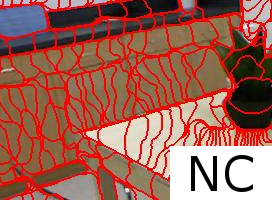
\includegraphics{../submission/pictures/nyu-test-1-nc-excerpt}
            }
            &
            \resizebox{\linewidth}{!}{
                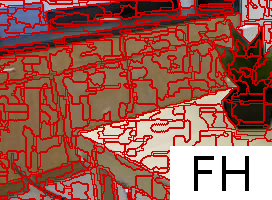
\includegraphics{../submission/pictures/nyu-test-1-fh-excerpt}
            }
            &
            \resizebox{\linewidth}{!}{
                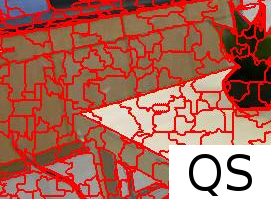
\includegraphics{../submission/pictures/nyu-test-1-qs-excerpt}
            }
            &
            \resizebox{\linewidth}{!}{
                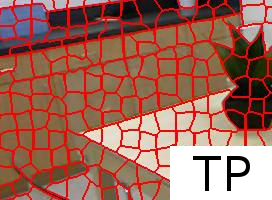
\includegraphics{../submission/pictures/nyu-test-1-tp-excerpt}
            }
            &
            \resizebox{\linewidth}{!}{
                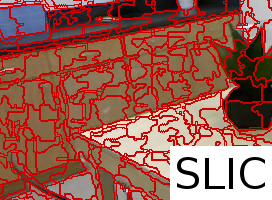
\includegraphics{../submission/pictures/nyu-test-1-orislic-excerpt}
            }
            &
            \resizebox{\linewidth}{!}{
                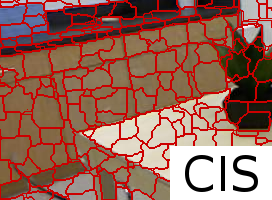
\includegraphics{../submission/pictures/nyu-test-1-cis-excerpt}
            }
            &
            \resizebox{\linewidth}{!}{
                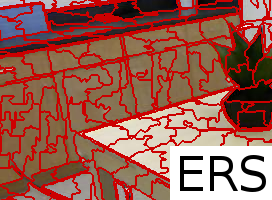
\includegraphics{../submission/pictures/nyu-test-1-ers-excerpt}
            }
            \\
            \resizebox{\linewidth}{!}{
                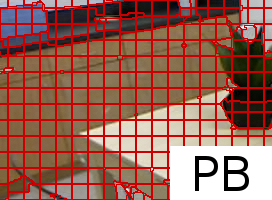
\includegraphics{../submission/pictures/nyu-test-1-pb-excerpt}
            }
            &
            \resizebox{\linewidth}{!}{
                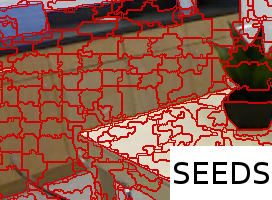
\includegraphics{../submission/pictures/nyu-test-1-oriseedsmp-excerpt}
            }
            &
            \resizebox{\linewidth}{!}{
                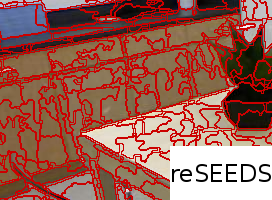
\includegraphics{../submission/pictures/nyu-test-1-reseedsmp-excerpt}
            }
            &
            \resizebox{\linewidth}{!}{
                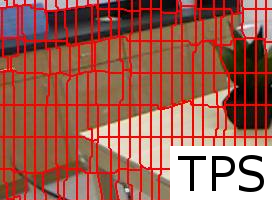
\includegraphics{../submission/pictures/nyu-test-1-tps-excerpt}
            }
            &
            \resizebox{\linewidth}{!}{
                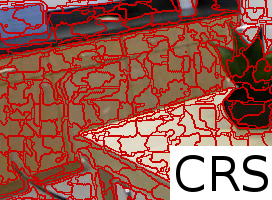
\includegraphics{../submission/pictures/nyu-test-1-crs-excerpt}
            }
            &
            \resizebox{\linewidth}{!}{
                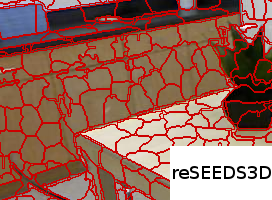
\includegraphics{../submission/pictures/nyu-test-1-seeds3d-excerpt}
            }
            &
            \resizebox{\linewidth}{!}{
                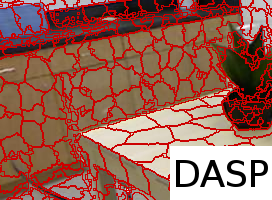
\includegraphics{../submission/pictures/nyu-test-1-dasp-beta-0-05-excerpt}
            }
            &
            \resizebox{\linewidth}{!}{
                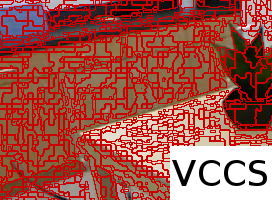
\includegraphics{../submission/pictures/nyu-test-1-vccs-excerpt}
            }            
        \end{tabularx}
        {\footnotesize Figure 2: Superpixel segmentations obtained on an image from the NYUV2.}
    }
    
    \headerbox{Qualitative Results (cont'd)}{name=qualitative,column=1,span=1}{
        \begin{tabularx}{\linewidth}{@{}Y@{}Y@{}Y@{}Y@{}Y@{}Y@{}Y@{}}
            \resizebox{0.99\linewidth}{!}{
                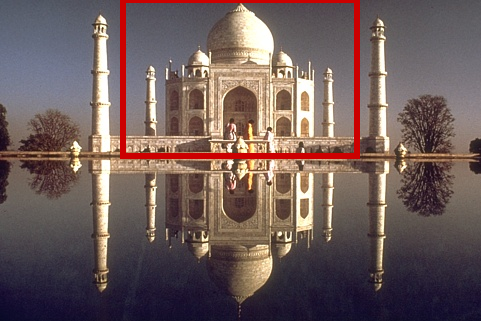
\includegraphics{pictures/bsd-test-3-excerpt}
            }
            &
            %\resizebox{\linewidth}{!}{
            %    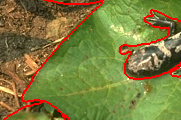
\includegraphics{../submission/pictures/bsd-test-2-contours-excerpt}
            %}
            %&
            \resizebox{\linewidth}{!}{
                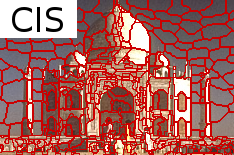
\includegraphics{pictures/bsd-test-3-cis-excerpt}
            }
            &
            \resizebox{\linewidth}{!}{
                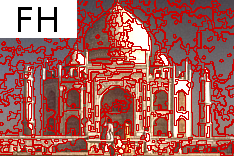
\includegraphics{pictures/bsd-test-3-fh-excerpt}
            }
            &
            \resizebox{\linewidth}{!}{
                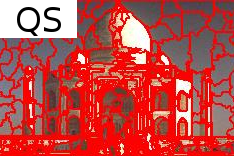
\includegraphics{pictures/bsd-test-3-qs-excerpt}
            }
            &
            \resizebox{\linewidth}{!}{
                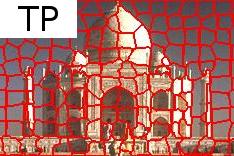
\includegraphics{pictures/bsd-test-3-tp-excerpt}
            }
            &
            \resizebox{\linewidth}{!}{
                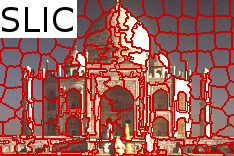
\includegraphics{pictures/bsd-test-3-orislic-excerpt}
            }
            &
            \resizebox{\linewidth}{!}{
                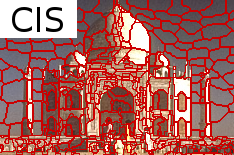
\includegraphics{pictures/bsd-test-3-cis-excerpt}
            }
            \\
            &
            \resizebox{\linewidth}{!}{
                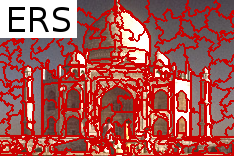
\includegraphics{pictures/bsd-test-3-ers-excerpt}
            }
            &
            \resizebox{\linewidth}{!}{
                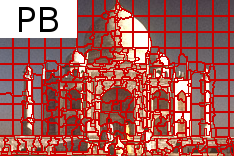
\includegraphics{pictures/bsd-test-3-pb-excerpt}
            }
            &
            \resizebox{\linewidth}{!}{
                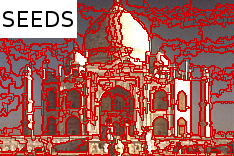
\includegraphics{pictures/bsd-test-3-oriseedsmp-excerpt}
            }
            &
            \resizebox{\linewidth}{!}{
                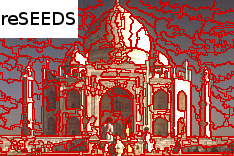
\includegraphics{pictures/bsd-test-3-reseedsmp-excerpt}
            }
            &
            \resizebox{\linewidth}{!}{
                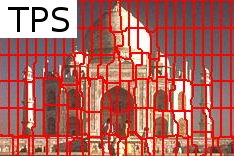
\includegraphics{pictures/bsd-test-3-tps-excerpt}
            }
            &
            \resizebox{\linewidth}{!}{
                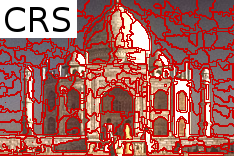
\includegraphics{pictures/bsd-test-3-crs-excerpt}
            }
        \end{tabularx}
        
        {\footnotesize Figure 3: Superpixel segmentations obtained on an image from the BSDS500.}
        \vskip 0.5em
        
        \begin{tabularx}{\linewidth}{@{}Y@{}Y@{}Y@{}Y@{}Y@{}Y@{}Y@{}Y@{}}
            \resizebox{0.99\linewidth}{!}{
                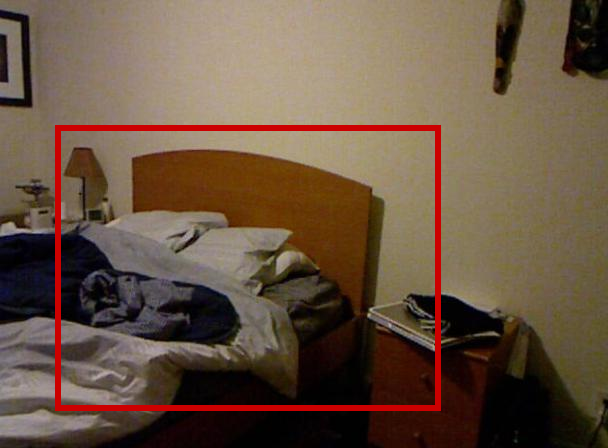
\includegraphics{pictures/nyu-test-2-excerpt}
            }
            &
            %\resizebox{\linewidth}{!}{
            %    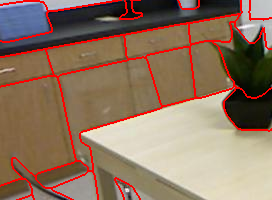
\includegraphics[scale=0.2016]{../submission/pictures/nyu-test-1-contours-excerpt}
            %}
            %&
            \resizebox{\linewidth}{!}{
                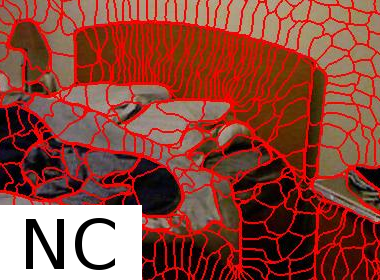
\includegraphics{pictures/nyu-test-2-nc-excerpt}
            }
            &
            \resizebox{\linewidth}{!}{
                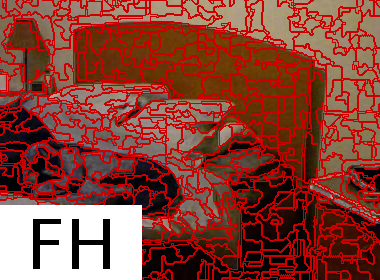
\includegraphics{pictures/nyu-test-2-fh-excerpt}
            }
            &
            \resizebox{\linewidth}{!}{
                \includegraphics{pictures/nyu-test-2-qs-excerpt}
            }
            &
            \resizebox{\linewidth}{!}{
                \includegraphics{pictures/nyu-test-2-tp-excerpt}
            }
            &
            \resizebox{\linewidth}{!}{
                \includegraphics{pictures/nyu-test-2-orislic-excerpt}
            }
            &
            \resizebox{\linewidth}{!}{
                \includegraphics{pictures/nyu-test-2-cis-excerpt}
            }
            &
            \resizebox{\linewidth}{!}{
                \includegraphics{pictures/nyu-test-2-ers-excerpt}
            }
            \\
            \resizebox{\linewidth}{!}{
                \includegraphics{pictures/nyu-test-2-pb-excerpt}
            }
            &
            \resizebox{\linewidth}{!}{
                \includegraphics{pictures/nyu-test-2-oriseedsmp-excerpt}
            }
            &
            \resizebox{\linewidth}{!}{
                \includegraphics{pictures/nyu-test-2-reseedsmp-excerpt}
            }
            &
            \resizebox{\linewidth}{!}{
                \includegraphics{pictures/nyu-test-2-tps-excerpt}
            }
            &
            \resizebox{\linewidth}{!}{
                \includegraphics{pictures/nyu-test-2-crs-excerpt}
            }
            &
            \resizebox{\linewidth}{!}{
                \includegraphics{pictures/nyu-test-2-seeds3d-excerpt}
            }
            &
            \resizebox{\linewidth}{!}{
                \includegraphics{pictures/nyu-test-2-dasp-beta-0-05-excerpt}
            }
            &
            \resizebox{\linewidth}{!}{
                \includegraphics{pictures/nyu-test-2-vccs-excerpt}
            }            
        \end{tabularx}
        {\footnotesize Figure 4: Superpixel segmentations obtained on an image from the NYUV2.}
    }
    
    \headerbox{Quantitative Results}{name=quantitative,column=1,span=1,below=qualitative}{
        
        \begin{tabularx}{\linewidth}{@{}Y@{}Y@{} !{\color{RWTHblue}\vrule} Y@{}Y@{}Y@{}}
            \resizebox{0.98\linewidth}{!}{
		        \begin{tikzpicture}
			        \begin{axis}[
					        height=7.3cm,
					        width=3cm,
					        y label style={at={(axis description cs:0.45,1.02)},anchor=south,rotate=-90},
					        xlabel=Superpixels,
					        xlabel shift={0.1cm},
					        ylabel=$Rec$ (BSDS500),
					        ymin=0.9,
					        ymax=1,
					        xmin=100,
					        xmax=1200,
					        xticklabel shift={.1cm},
					        xtick={400,1000},
					        yticklabel shift={.1cm},
					        cycle list name=comparison bsd]
					
				        % NC
				        \addplot+[thick] table [row sep=newline,trim cells=true,x=K,y=Rec] {../submission/data/nc-bsd.csv};
				        \label{plot:evaluation-comparison-nc-rec-bsd}
				
				        % FH
				        \addplot+[thick] table [row sep=newline,trim cells=true,x=K,y=Rec] {../submission/data/fh-bsd-test.csv};
				        \label{plot:evaluation-comparison-fh-rec-bsd}
				
				        % QS
				        \addplot+[thick] table [row sep=newline,trim cells=true,x=K,y=Rec] {../submission/data/qs-bsd-test.csv};
				        \label{plot:evaluation-comparison-qs-rec-bsd}
				
				        % TP
				        \addplot+[thick] table [row sep=newline,trim cells=true,x=K,y=Rec] {../submission/data/tp-bsd-test.csv};
				        \label{plot:evaluation-comparison-tp-rec-bsd}
				
				        % oriSLIC
				        \addplot+[thick] table [row sep=newline,trim cells=true,x=K,y=Rec] {../submission/data/orislic-bsd-test.csv};
				        \label{plot:evaluation-comparison-orislic-rec-bsd}
				
				        % CIS
				        \addplot+[thick] table [row sep=newline,trim cells=true,x=K,y=Rec] {../submission/data/cis-bsd-test.csv};
				        \label{plot:evaluation-comparison-cis-rec-bsd}
				
				        % ERS
				        \addplot+[thick] table [row sep=newline,trim cells=true,x=K,y=Rec] {../submission/data/ers-bsd-test.csv};
				        \label{plot:evaluation-comparison-ers-rec-bsd}
				
				        % PB
				        \addplot+[thick] table [row sep=newline,trim cells=true,x=K,y=Rec] {../submission/data/pb-bsd-test.csv};
				        \label{plot:evaluation-comparison-pb-rec-bsd}
				
				        % SEEDSmp
				        \addplot+[thick] table [row sep=newline,trim cells=true,x=K,y=Rec] {../submission/data/oriseedsmp-bsd-test.csv};
				        \label{plot:evaluation-comparison-oriseedsmp-rec-bsd}
				
                        % reSEEDSmp
				        \addplot+[thick] table [row sep=newline,trim cells=true,x=K,y=Rec] {../submission/data/reseedsmp-bsd-test.csv};
				        \label{plot:evaluation-comparison-reseedssm-rec-bsd}

				        % reSEEDSmp*
				        %\addplot+[thick] table [row sep=newline,trim cells=true,x=K,y=Rec] {../submission/data/reseedssm-bsd-test.csv};
				        %\label{plot:evaluation-comparison-reseedssm-rec-bsd}
				
				        % TPS
				        \addplot+[thick] table [row sep=newline,trim cells=true,x=K,y=Rec] {../submission/data/tps-bsd-test.csv};
				        \label{plot:evaluation-comparison-tps-rec-bsd}
				
				        % CRS
				        \addplot+[thick] table [row sep=newline,trim cells=true,x=K,y=Rec] {../submission/data/crs-bsd-test.csv};
				        \label{plot:evaluation-comparison-crs-rec-bsd}
			        \end{axis}
		        \end{tikzpicture}
		    }
	        &
	        \resizebox{0.98\linewidth}{!}{
		        \begin{tikzpicture}
			        \begin{axis}[
					        height=7.3cm,
					        width=3cm,
					        y label style={at={(axis description cs:0.45,1.02)},anchor=south,rotate=-90},
					        xlabel=Superpixels,
					        xlabel shift={0.1cm},
					        ylabel=$UE$ (BSDS500),
					        ymin=0.025,
					        ymax=0.1,
					        xmin=100,
					        xmax=1200,
					        xticklabel shift={.1cm},
					        xtick={400,1000},
					        yticklabel shift={.1cm},
					        cycle list name=comparison bsd]
				
				        % NC
				        \addplot+[thick] table [row sep=newline,trim cells=true,x=K,y=UE] {../submission/data/nc-bsd.csv};
				        \label{plot:evaluation-comparison-nc-ue-bsd}
				
				        % FH
				        \addplot+[thick] table [row sep=newline,trim cells=true,x=K,y=UE] {../submission/data/fh-bsd-test.csv};
				        \label{plot:evaluation-comparison-fh-ue-bsd}
				
				        % QS
				        \addplot+[thick] table [row sep=newline,trim cells=true,x=K,y=UE] {../submission/data/qs-bsd-test.csv};
				        \label{plot:evaluation-comparison-qs-ue-bsd}
				
				        % TP
				        \addplot+[thick] table [row sep=newline,trim cells=true,x=K,y=UE] {../submission/data/tp-bsd-test.csv};
				        \label{plot:evaluation-comparison-tp-ue-bsd}
				
				        % oriSLIC
				        \addplot+[thick] table [row sep=newline,trim cells=true,x=K,y=UE] {../submission/data/orislic-bsd-test.csv};
				        \label{plot:evaluation-comparison-orislic-ue-bsd}
				
				        % CIS
				        \addplot+[thick] table [row sep=newline,trim cells=true,x=K,y=UE] {../submission/data/cis-bsd-test.csv};
				        \label{plot:evaluation-comparison-cis-ue-bsd}
				
				        % ERS
				        \addplot+[thick] table [row sep=newline,trim cells=true,x=K,y=UE] {../submission/data/ers-bsd-test.csv};
				        \label{plot:evaluation-comparison-ers-ue-bsd}
				
				        % PB
				        \addplot+[thick] table [row sep=newline,trim cells=true,x=K,y=UE] {../submission/data/pb-bsd-test.csv};
				        \label{plot:evaluation-comparison-pb-ue-bsd}
				
				        % SEEDSmp
				        \addplot+[thick] table [row sep=newline,trim cells=true,x=K,y=UE] {../submission/data/oriseedsmp-bsd-test.csv};
				        \label{plot:evaluation-comparison-oriseedsmp-ue-bsd}
				
				        % reSEEDSmp
				        \addplot+[thick] table [row sep=newline,trim cells=true,x=K,y=UE] {../submission/data/reseedsmp-bsd-test.csv};
				        \label{plot:evaluation-comparison-reseedssm-ue-bsd}
				
                        % reSEEDSmp*
				        %\addplot+[thick] table [row sep=newline,trim cells=true,x=K,y=UE] {../submission/data/reseedssm-bsd-test.csv};
				        %\label{plot:evaluation-comparison-reseedssm-ue-bsd}

				        % TPS
				        \addplot+[thick] table [row sep=newline,trim cells=true,x=K,y=UE] {../submission/data/tps-bsd-test.csv};
				        \label{plot:evaluation-comparison-tps-ue-bsd}
				
				        % CRS
				        \addplot+[thick] table [row sep=newline,trim cells=true,x=K,y=UE] {../submission/data/crs-bsd-test.csv};
				        \label{plot:evaluation-comparison-crs-ue-bsd}
			        \end{axis}
		        \end{tikzpicture}
		    }
	        &
	        \resizebox{\linewidth}{!}{
		        \begin{tikzpicture}
			        \begin{axis}[
					        height=7.3cm,
					        width=3cm,
					        y label style={at={(axis description cs:0.4,1.02)},anchor=south,rotate=-90},
					        xlabel=Superpixels,
					        xlabel shift={0.1cm},
					        ylabel=$Rec$ (NYUV2),
					        ymin=0.9,
					        ymax=1,
					        xmin=300,
					        xmax=1700,
					        xticklabel shift={.1cm},
					        xtick={500,1500},
					        yticklabel shift={.1cm},
					        cycle list name=comparison nyu]
				
				        % NC
				        \addplot+[thick] table [row sep=newline,trim cells=true,x=K,y=Rec] {../submission/data/nc-nyu.csv};
				        \label{plot:evaluation-comparison-nc-rec-nyu}
				
				        % FH
				        \addplot+[thick] table [row sep=newline,trim cells=true,x=K,y=Rec] {../submission/data/fh-nyu-test.csv};
				        \label{plot:evaluation-comparison-fh-rec-nyu}
				
				        % QS
				        \addplot+[thick] table [row sep=newline,trim cells=true,x=K,y=Rec] {../submission/data/qs-nyu-test.csv};
				        \label{plot:evaluation-comparison-qs-rec-nyu}
				
				        % TP
				        \addplot+[thick] table [row sep=newline,trim cells=true,x=K,y=Rec] {../submission/data/tp-nyu-test.csv};
				        \label{plot:evaluation-comparison-tp-rec-nyu}
				
				        % oriSLIC
				        \addplot+[thick] table [row sep=newline,trim cells=true,x=K,y=Rec] {../submission/data/orislic-nyu-test.csv};
				        \label{plot:evaluation-comparison-orislic-rec-nyu}
				
				        % SLIC3D
				        %\addplot+[thick] table [row sep=newline,trim cells=true,x=K,y=Rec] {../submission/data/slic3d-nyu-test.csv};
				        %\label{plot:evaluation-comparison-slic3d-rec-nyu}
				
				        % CIS
				        \addplot+[thick] table [row sep=newline,trim cells=true,x=K,y=Rec] {../submission/data/cis-nyu-test.csv};
				        \label{plot:evaluation-comparison-cis-rec-nyu}
				
				        % ERS
				        \addplot+[thick] table [row sep=newline,trim cells=true,x=K,y=Rec] {../submission/data/ers-nyu-test.csv};
				        \label{plot:evaluation-comparison-ers-rec-nyu}
				
				        % PB
				        \addplot+[thick] table [row sep=newline,trim cells=true,x=K,y=Rec] {../submission/data/pb-nyu-test.csv};
				        \label{plot:evaluation-comparison-pb-rec-nyu}
				
				        % SEEDSmp
				        \addplot+[thick] table [row sep=newline,trim cells=true,x=K,y=Rec] {../submission/data/oriseedsmp-nyu-test.csv};
				        \label{plot:evaluation-comparison-oriseedsmp-rec-nyu}
				
                        % reSEEDSmp
				        \addplot+[thick] table [row sep=newline,trim cells=true,x=K,y=Rec] {../submission/data/reseedsmp-nyu-test.csv};
				        \label{plot:evaluation-comparison-reseedssm-rec-nyu}

				        % reSEEDSmp*
				        %\addplot+[thick] table [row sep=newline,trim cells=true,x=K,y=Rec] {../submission/data/reseedssm-nyu-test.csv};
				        %\label{plot:evaluation-comparison-reseedssm-rec-nyu}
				
				        % reSEEDS3D
				        \addplot+[thick] table [row sep=newline,trim cells=true,x=K,y=Rec] {../submission/data/seeds3d-nyu-test.csv};
				        \label{plot:evaluation-comparison-seeds3d-rec-nyu}
				
				        % DASP
				        \addplot+[thick] table [row sep=newline,trim cells=true,x=K,y=Rec] {../submission/data/dasp-nyu-test.csv};
				        \label{plot:evaluation-comparison-dasp-rec-nyu}
				
				        % TPS
				        \addplot+[thick] table [row sep=newline,trim cells=true,x=K,y=Rec] {../submission/data/tps-nyu-test.csv};
				        \label{plot:evaluation-comparison-tps-rec-nyu}
				
				        % CRS
				        \addplot+[thick] table [row sep=newline,trim cells=true,x=K,y=Rec] {../submission/data/crs-nyu-test.csv};
				        \label{plot:evaluation-comparison-crs-rec-nyu}
				
				        % DCRS
				
				        % VCCS
				        \addplot+[thick] table [row sep=newline,trim cells=true,x=K,y=Rec] {../submission/data/vccs-depth-test.csv};
				        \label{plot:evaluation-comparison-vccs-rec-nyu}
			        \end{axis}
		        \end{tikzpicture}
		    }
	        &
	        \resizebox{\linewidth}{!}{
		        \begin{tikzpicture}
			        \begin{axis}[
					        height=7.3cm,
					        width=3cm,
					        y label style={at={(axis description cs:0.4,1.02)},anchor=south,rotate=-90},
					        xlabel=Superpixels,
					        xlabel shift={0.1cm},
					        ylabel=$UE$ (NYUV2),
					        ymin=0.07,
					        ymax=0.17,
					        xmin=300,
					        xmax=1700,
					        xticklabel shift={.1cm},
					        xtick={500,1500},
					        yticklabel shift={.1cm},
					        cycle list name=comparison nyu]
				
				        % NC
				        \addplot+[thick] table [row sep=newline,trim cells=true,x=K,y=UE] {../submission/data/nc-nyu.csv};
				        \label{plot:evaluation-comparison-nc-ue-nyu}
				
				        % FH
				        \addplot+[thick] table [row sep=newline,trim cells=true,x=K,y=UE] {../submission/data/fh-nyu-test.csv};
				        \label{plot:evaluation-comparison-fh-ue-nyu}
				
				        % QS
				        \addplot+[thick] table [row sep=newline,trim cells=true,x=K,y=UE] {../submission/data/qs-nyu-test.csv};
				        \label{plot:evaluation-comparison-qs-ue-nyu}
				
				        % TP
				        \addplot+[thick] table [row sep=newline,trim cells=true,x=K,y=UE] {../submission/data/tp-nyu-test.csv};
				        \label{plot:evaluation-comparison-tp-ue-nyu}
				
				        % oriSLIC
				        \addplot+[thick] table [row sep=newline,trim cells=true,x=K,y=UE] {../submission/data/orislic-nyu-test.csv};
				        \label{plot:evaluation-comparison-orislic-ue-nyu}
				
				        % SLIC3D
				        %\addplot+[thick] table [row sep=newline,trim cells=true,x=K,y=UE] {../submission/data/slic3d-nyu-test.csv};
				        %\label{plot:evaluation-comparison-slic3d-ue-nyu}
				
				        % CIS
				        \addplot+[thick] table [row sep=newline,trim cells=true,x=K,y=UE] {../submission/data/cis-nyu-test.csv};
				        \label{plot:evaluation-comparison-cis-ue-nyu}
				
				        % ERS
				        \addplot+[thick] table [row sep=newline,trim cells=true,x=K,y=UE] {../submission/data/ers-nyu-test.csv};
				        \label{plot:evaluation-comparison-ers-ue-nyu}
				
				        % PB
				        \addplot+[thick] table [row sep=newline,trim cells=true,x=K,y=UE] {../submission/data/pb-nyu-test.csv};
				        \label{plot:evaluation-comparison-pb-ue-nyu}
				
				        % SEEDSmp
				        \addplot+[thick] table [row sep=newline,trim cells=true,x=K,y=UE] {../submission/data/oriseedsmp-nyu-test.csv};
				        \label{plot:evaluation-comparison-oriseedsmp-ue-nyu}
				
				        % reSEEDSmp
				        \addplot+[thick] table [row sep=newline,trim cells=true,x=K,y=UE] {../submission/data/reseedsmp-nyu-test.csv};
				        \label{plot:evaluation-comparison-reseedssm-ue-nyu}
				
				        % reSEEDSmp*
				        %\addplot+[thick] table [row sep=newline,trim cells=true,x=K,y=UE] {../submission/data/reseedssm-nyu-test.csv};
				        %\label{plot:evaluation-comparison-reseedssm-ue-nyu}
				
				        % reSEEDS3D
				        \addplot+[thick] table [row sep=newline,trim cells=true,x=K,y=UE] {../submission/data/seeds3d-nyu-test.csv};
				        \label{plot:evaluation-comparison-seeds3d-ue-nyu}
				
				        % DASP
				        \addplot+[thick] table [row sep=newline,trim cells=true,x=K,y=UE] {../submission/data/dasp-nyu-test.csv};
				        \label{plot:evaluation-comparison-dasp-ue-nyu}
				
				        % TPS
				        \addplot+[thick] table [row sep=newline,trim cells=true,x=K,y=UE] {../submission/data/tps-nyu-test.csv};
				        \label{plot:evaluation-comparison-tps-ue-nyu}
				
				        % CRS
				        \addplot+[thick] table [row sep=newline,trim cells=true,x=K,y=UE] {../submission/data/crs-nyu-test.csv};
				        \label{plot:evaluation-comparison-crs-ue-nyu}
				
				        % DCRS
				
				        % VCCS
				        \addplot+[thick] table [row sep=newline,trim cells=true,x=K,y=UE] {../submission/data/vccs-depth-test.csv};
				        \label{plot:evaluation-comparison-vccs-ue-nyu}
			        \end{axis}
		        \end{tikzpicture}
		    }
	    \end{tabularx}
	    
	    {\footnotesize Figure 5: Average Boundary Recall and Undersegmentation Error on the test sets of\\[-2pt] the BSDS500 (left) and the NYUV2 (right); parameters have been optimized on the\\[-2pt] corresponding training sets using discrete grid search.}
    }
    
    \headerbox{Runtime}{name=runtime,column=1,span=1,below=quantitative}{
        \begin{tabularx}{\linewidth}{@{}Y@{}Y@{}Y@{}Y@{}}
	        \resizebox{\linewidth}{!}{
		        \begin{tikzpicture}
			        \begin{axis}[
					        height=3.91cm,
					        width=3.75cm,
					        y label style={at={(axis description cs:0.25,1.04)},anchor=south,rotate=-90},
					        xlabel=Superpixels,
					        xlabel shift={0.1cm},
					        ylabel=$Rec$ (NYUV2),
					        ymin=0.9,
					        ymax=1,
					        xmin=300,
					        xmax=1700,
					        xtick={500,1500},
					        xticklabel shift={.1cm},
					        yticklabel shift={.1cm},
					        cycle list name=runtime nyu]
				
				        % FH
				        \addplot+[thick] table [row sep=newline,trim cells=true,x=K,y=Rec] {../submission/data/fh-nyu-test.csv};
				        \label{plot:evaluation-comparison-iteration-fh-rec-nyu}
				
				        % oriSLIC 1it
				        \addplot+[thick] table [row sep=newline,trim cells=true,x=K,y=Rec] {../submission/data/orislic1it-nyu-test.csv};
				        \label{plot:evaluation-comparison-iteration-orislic1it-rec-nyu}
				        
				        % oriSLIC
				        \addplot+[thick] table [row sep=newline,trim cells=true,x=K,y=Rec] {../submission/data/orislic-nyu-test.csv};
				        \label{plot:evaluation-comparison-orislic-rec-nyu}
				        
				        % SEEDSmp 1it
				        \addplot+[thick] table [row sep=newline,trim cells=true,x=K,y=Rec] {../submission/data/oriseedsmp1it-nyu-test.csv};
				        \label{plot:evaluation-comparison-iteration-oriseedsmp1it-rec-nyu}
				
				        % SEEDSmp
				        \addplot+[thick] table [row sep=newline,trim cells=true,x=K,y=Rec] {../submission/data/oriseedsmp-nyu-test.csv};
				        \label{plot:evaluation-comparison-iteration-oriseedsmp-rec-nyu}
				
				        % reSEEDSmp
				        %\addplot+[thick] table [row sep=newline,trim cells=true,x=K,y=Rec] {../submission/data/reseedsmp1it-nyu-test.csv};
				        %\label{plot:evaluation-comparison-iteration-reseedsmp-rec-nyu}
				
				        % reSEEDSmp 1it
				        \addplot+[thick] table [row sep=newline,trim cells=true,x=K,y=Rec] {../submission/data/reseedsmp1it-nyu-test.csv};
				        \label{plot:evaluation-comparison-iteration-reseedssm1it-rec-nyu}
				
				        % reSEEDSmp* 1it
				        %\addplot+[thick] table [row sep=newline,trim cells=true,x=K,y=Rec] {../submission/data/reseedssm1it-nyu-test.csv};
				        %\label{plot:evaluation-comparison-iteration-reseedssm1it-rec-nyu}
				
				        % reSEEDSmp
				        \addplot+[thick] table [row sep=newline,trim cells=true,x=K,y=Rec] {../submission/data/reseedsmp-nyu-test.csv};
				        \label{plot:evaluation-comparison-iteration-reseedssm-rec-nyu}
				
				        % reSEEDSmp*
				        %\addplot+[thick] table [row sep=newline,trim cells=true,x=K,y=Rec] {../submission/data/reseedssm-nyu-test.csv};
				        %\label{plot:evaluation-comparison-iteration-reseedssm-rec-nyu}
				
				        % reSEEDS3D
				        \addplot+[thick] table [row sep=newline,trim cells=true,x=K,y=Rec] {../submission/data/seeds3d1it-nyu-test.csv};
				        \label{plot:evaluation-comparison-iteration-seeds3d-rec-nyu}
				
				        % DASP
				        \addplot+[thick] table [row sep=newline,trim cells=true,x=K,y=Rec] {../submission/data/dasp-nyu-test.csv};
				        \label{plot:evaluation-comparison-iteration-dasp-rec-nyu}
				
				        % VCCS
				        \addplot+[thick] table [row sep=newline,trim cells=true,x=K,y=Rec] {../submission/data/vccs-depth-test.csv};
				        \label{plot:evaluation-comparison-iteration-vccs-rec-nyu}
				
			        \end{axis}
		        \end{tikzpicture}
		    }
		    &
		    \resizebox{\linewidth}{!}{
		        \begin{tikzpicture}
			        \begin{axis}[
					        height=3.91cm,
					        width=3.75cm,
					        y label style={at={(axis description cs:0.25,1.04)},anchor=south,rotate=-90},
					        xlabel=Superpixels,
					        xlabel shift={0.1cm},
					        ylabel=$UE$ (NYUV2),
					        ymin=0.07,
					        ymax=0.17,
					        xmin=300,
					        xmax=1700,
					        xtick={500,1500},
					        xticklabel shift={.1cm},
					        yticklabel shift={.1cm},
					        cycle list name=runtime nyu]
				
				        % FH
				        \addplot+[thick] table [row sep=newline,trim cells=true,x=K,y=UE] {../submission/data/fh-nyu-test.csv};
				        \label{plot:evaluation-comparison-iteration-fh-ue-nyu}
				
				        % oriSLIC 1it
				        \addplot+[thick] table [row sep=newline,trim cells=true,x=K,y=UE] {../submission/data/orislic1it-nyu-test.csv};
				        \label{plot:evaluation-comparison-iteration-orislic1it-ue-nyu}
				
				        % oriSLIC
				        \addplot+[thick] table [row sep=newline,trim cells=true,x=K,y=UE] {../submission/data/orislic-nyu-test.csv};
				        \label{plot:evaluation-comparison-iteration-orislic-ue-nyu}
				
				        % SLIC3D
				        %\addplot+[thick] table [row sep=newline,trim cells=true,x=K,y=UE] {../submission/data/slic3d-nyu-test.csv};
				        %\label{plot:evaluation-comparison-slic3d-ue-nyu}
				
				        % SEEDSmp 1it
				        \addplot+[thick] table [row sep=newline,trim cells=true,x=K,y=UE] {../submission/data/oriseedsmp1it-nyu-test.csv};
				        \label{plot:evaluation-comparison-iteration-oriseedsmp1it-ue-nyu}
				
				        % SEEDSmp
				        \addplot+[thick] table [row sep=newline,trim cells=true,x=K,y=UE] {../submission/data/oriseedsmp-nyu-test.csv};
				        \label{plot:evaluation-comparison-iteration-oriseedsmp-ue-nyu}
				
				        % reSEEDSmp
				        %\addplot+[thick] table [row sep=newline,trim cells=true,x=K,y=UE] {../submission/data/reseedsmp1it-nyu-test.csv};
				        %\label{plot:evaluation-comparison-iteration-reseedsmp-ue-nyu}
				
				        % reSEEDSmp 1it
				        \addplot+[thick] table [row sep=newline,trim cells=true,x=K,y=UE] {../submission/data/reseedsmp1it-nyu-test.csv};
				        \label{plot:evaluation-comparison-iteration-reseedssm1it-ue-nyu}
				
				        % reSEEDSmp* 1it
				        %\addplot+[thick] table [row sep=newline,trim cells=true,x=K,y=UE] {../submission/data/reseedssm1it-nyu-test.csv};
				        %\label{plot:evaluation-comparison-iteration-reseedssm1it-ue-nyu}
				
				        % reSEEDSmp
				        \addplot+[thick] table [row sep=newline,trim cells=true,x=K,y=UE] {../submission/data/reseedsmp-nyu-test.csv};
				        \label{plot:evaluation-comparison-iteration-reseedssm-ue-nyu}
				
				        % reSEEDSmp*
				        %\addplot+[thick] table [row sep=newline,trim cells=true,x=K,y=UE] {../submission/data/reseedssm-nyu-test.csv};
				        %\label{plot:evaluation-comparison-iteration-reseedssm-ue-nyu}
				
				        % reSEEDS3D
				        \addplot+[thick] table [row sep=newline,trim cells=true,x=K,y=UE] {../submission/data/seeds3d1it-nyu-test.csv};
				        \label{plot:evaluation-comparison-iteration-seeds3d-ue-nyu}
				
				        % DASP
				        \addplot+[thick] table [row sep=newline,trim cells=true,x=K,y=UE] {../submission/data/dasp-nyu-test.csv};
				        \label{plot:evaluation-comparison-iteration-dasp-ue-nyu}
				
				        % VCCS
				        \addplot+[thick] table [row sep=newline,trim cells=true,x=K,y=UE] {../submission/data/vccs-depth-test.csv};
				        \label{plot:evaluation-comparison-iteration-vccs-ue-nyu}
				
			        \end{axis}
		        \end{tikzpicture}
	        }
	        &
	        \resizebox{\linewidth}{!}{
		        \begin{tikzpicture}
			        \begin{axis}[
					        height=3.8cm,
					        width=3.75cm,
					        y label style={at={(axis description cs:0.275,1.04)},anchor=south,rotate=-90},
					        xlabel=Superpixels,
					        xlabel shift={0.1cm},
					        ylabel=$t$ in $s$ (NYUV2),
					        ymin=0,
					        ymax=0.45,
					        xmin=300,
					        xmax=1700,
					        xtick={500,1500},
					        xticklabel shift={.1cm},
					        yticklabel shift={.1cm},
					        cycle list name=runtime nyu]
				
				        % FH
				        \addplot+[thick] table [row sep=newline,trim cells=true,x=K,y=t] {../submission/data/fh-nyu-test.csv};
				        \label{plot:evaluation-comparison-iteration-fh-t-nyu}
				
				        % oriSLIC 1it
				        \addplot+[thick] table [row sep=newline,trim cells=true,x=K,y=t] {../submission/data/orislic1it-nyu-test.csv};
				        \label{plot:evaluation-comparison-iteration-orislic1it-t-nyu}
				
				        % oriSLIC
				        \addplot+[thick] table [row sep=newline,trim cells=true,x=K,y=t] {../submission/data/orislic-nyu-test.csv};
				        \label{plot:evaluation-comparison-iteration-orislic-t-nyu}
				
				        % SEEDSmp 1it
				        \addplot+[thick] table [row sep=newline,trim cells=true,x=K,y=t] {../submission/data/oriseedsmp1it-nyu-test.csv};
				        \label{plot:evaluation-comparison-iteration-oriseedsmp1it-t-nyu}
				
				        % SEEDSmp
				        \addplot+[thick] table [row sep=newline,trim cells=true,x=K,y=t] {../submission/data/oriseedsmp-nyu-test.csv};
				        \label{plot:evaluation-comparison-iteration-oriseedsmp-t-nyu}
				
				        % reSEEDSmp 1it
				        \addplot+[thick] table [row sep=newline,trim cells=true,x=K,y=t] {../submission/data/reseedsmp1it-nyu-test.csv};
				        \label{plot:evaluation-comparison-iteration-reseedssm1it-t-nyu}
				
				        % reSEEDSmp* 1it
				        %\addplot+[thick] table [row sep=newline,trim cells=true,x=K,y=t] {../submission/data/reseedssm1it-nyu-test.csv};
				        %\label{plot:evaluation-comparison-iteration-reseedssm1it-t-nyu}
				
				        % reSEEDSmp
				        \addplot+[thick] table [row sep=newline,trim cells=true,x=K,y=t] {../submission/data/reseedsmp-nyu-test.csv};
				        \label{plot:evaluation-comparison-iteration-reseedssm-t-nyu}
				
				        % reSEEDSmp*
				        %\addplot+[thick] table [row sep=newline,trim cells=true,x=K,y=t] {../submission/data/reseedssm-nyu-test.csv};
				        %\label{plot:evaluation-comparison-iteration-reseedssm-t-nyu}
				
				        % reSEEDS3D
				        \addplot+[thick] table [row sep=newline,trim cells=true,x=K,y=t] {../submission/data/seeds3d-nyu-test.csv};
				        \label{plot:evaluation-comparison-iteration-seeds3d-t-nyu}
				
				        % DASP
				        \addplot+[thick] table [row sep=newline,trim cells=true,x=K,y=t] {../submission/data/dasp-nyu-test.csv};
				        \label{plot:evaluation-comparison-iteration-dasp-t-nyu}
				
				        % VCCS
				        \addplot+[thick] table [row sep=newline,trim cells=true,x=K,y=t] {../submission/data/vccs-depth-test.csv};
				        \label{plot:evaluation-comparison-iteration-vccs-t-nyu}
			        \end{axis}
		        \end{tikzpicture}
		    }
	    \end{tabularx}
	    
	    {\footnotesize Figure 6: Average Boundary Recall, Undersegmentation Error and runtime on the test\\[-2pt] set of the NYUV2; $^\star$ marks algorithms optimized for low runtime:\\[-2pt] \ref{plot:evaluation-comparison-iteration-orislic1it-t-nyu} \textbf{SLIC} $^\star$; \ref{plot:evaluation-comparison-iteration-oriseedsmp1it-t-nyu} \textbf{SEEDS} $^\star$; \ref{plot:evaluation-comparison-iteration-reseedssm1it-t-nyu} \textbf{reSEEDS} $^\star$.}
    }
    
    \headerbox{Conclusion}{name=conclusion,column=1,span=1,below=runtime}{
        In conclusion, several algorithms demonstrate excellent performance and low runtime. Furthermore, using depth information does not improve performance in all cases (e.g. \textbf{DASP}, \textbf{reSEEDS3D}). However, directly segmenting point clouds turns out to be advantageous (e.g. \textbf{VCCS}). While additional aspects may be necessary to asses superpixel algorithms with regard to specific applications, the presented results offer a general overview and allow to select suitable superpixel algorithms for a wide range of applications.
        
        %\vskip 4px
        %Code and further results available at {\ttfamily \bfseries davidstutz.de}.
        
        \begin{minipage}{0.825\textwidth}
            Further results and source code: {\ttfamily \bfseries davidstutz.de}
            \vskip 4px
            
            Acknowledgments:\\Alexander Hermans, Prof. Dr. Bastian Leibe
            \vfill
        \end{minipage}
        \begin{minipage}{0.15\textwidth}
            \includegraphics[scale=0.15]{qrcode}
        \end{minipage}
    }
	
\end{poster}
\end{document}
